\documentclass[12pt, a4paper]{article}
\usepackage[utf8]{inputenc}
\usepackage[T1]{fontenc}
\usepackage[brazil]{babel}
\usepackage{amsmath, amsfonts, amssymb}
\usepackage{graphicx}
\usepackage{geometry}
\usepackage{setspace}
\usepackage{indentfirst}
\usepackage{caption}
\usepackage{subcaption}
\usepackage{cite}
\usepackage{listings}
\usepackage[dvipsnames,table]{xcolor}
\usepackage{booktabs}
\usepackage{array}
\usepackage{multirow}
\usepackage{fancyhdr}
\usepackage{hyperref}
\usepackage{siunitx}
\usepackage{mathtools}
\usepackage{float}
\usepackage{enumitem}
\usepackage{mdframed}
\usepackage{tcolorbox}
\tcbuselibrary{skins,breakable}
\usepackage{tikz}
\usetikzlibrary{shapes.geometric,arrows.meta,positioning,fit,backgrounds,calc}

\geometry{left=3cm, top=3cm, right=2cm, bottom=2cm}
\onehalfspacing

% ─── Cores ────────────────────────────────────────────────────────────────────
\definecolor{codegray}{rgb}{0.96,0.96,0.96}
\definecolor{codeblue}{rgb}{0.0,0.0,0.6}
\definecolor{codegreen}{rgb}{0.0,0.45,0.0}
\definecolor{codepurple}{rgb}{0.5,0.0,0.6}
\definecolor{codered}{rgb}{0.6,0.0,0.0}
\definecolor{aquacolor}{rgb}{0.0,0.50,0.55}
\definecolor{boxblue}{rgb}{0.88,0.93,0.98}
\definecolor{boxgreen}{rgb}{0.88,0.97,0.88}
\definecolor{boxyellow}{rgb}{1.0,0.98,0.88}

% ─── Listagens de codigo ──────────────────────────────────────────────────────
\lstset{
  basicstyle=\ttfamily\footnotesize,
  backgroundcolor=\color{codegray},
  frame=single, rulecolor=\color{gray!50},
  breaklines=true,
  keywordstyle=\color{codeblue}\bfseries,
  commentstyle=\color{codegreen}\itshape,
  stringstyle=\color{codepurple},
  numbers=left, numberstyle=\tiny\color{gray}, numbersep=6pt,
  tabsize=2, showspaces=false, showstringspaces=false,
  captionpos=b,
}

% ─── Caixas de destaque ───────────────────────────────────────────────────────
\newtcolorbox{conceitobox}[1][]{
  colback=boxblue, colframe=aquacolor!80!black,
  fonttitle=\bfseries, title=#1, breakable, before upper=\setlength{\parskip}{4pt}
}
\newtcolorbox{resultadobox}[1][]{
  colback=boxgreen, colframe=codegreen!70!black,
  fonttitle=\bfseries, title=#1, breakable
}
\newtcolorbox{unidadebox}[1][]{
  colback=boxyellow, colframe=orange!70!black,
  fonttitle=\bfseries\small, title=#1, breakable,
  before upper=\footnotesize
}

% ─── Cabecalho ────────────────────────────────────────────────────────────────
\pagestyle{fancy}\fancyhf{}
\rhead{\footnotesize Aqua Monitor -- Comparador de Tensao -- PADIS U7/C5}
\lhead{\footnotesize Engenharia da Computacao | Microeletronica}
\rfoot{\thepage}

\hypersetup{colorlinks=true, linkcolor=aquacolor!80!black,
            citecolor=codeblue, urlcolor=codeblue}

\begin{document}

%% ──────────────────────────────────────────────────────────────────────────────
%%  CAPA
%% ──────────────────────────────────────────────────────────────────────────────
\begin{titlepage}
\begin{center}
  {\Large\bfseries Universidade Federal do Amazonas -- UFAM}\\[0.2cm]
  {\large\bfseries Faculdade de Tecnologia -- FT}\\[0.1cm]
  {\large\bfseries Curso de Engenharia da Computacao}\\[1.8cm]

  {\large\bfseries Matheus Serrao Uchoa}\\[1.8cm]

  {\LARGE\bfseries RELATORIO TECNICO\\[0.3cm]
   PADIS -- Unidade 7 $|$ Capitulo 5}\\[0.7cm]

  {\Large\bfseries Comparador de Tensao para SAR ADC de 4~Bits\\[0.3cm]
   Projeto AquaMonitor\\[0.3cm]
   Tecnologia CMOS TSMC 0{,}18~$\mu$m}\\[2.0cm]

  \vfill
  {\normalsize\textbf{Professor:} Thiago Brito}\\[0.15cm]
  {\normalsize\textbf{Disciplina:} Design de Circuitos Integrados (CI Amazonia)}\\[0.15cm]
  {\normalsize Manaus -- AM \quad Maio de 2026}
\end{center}
\end{titlepage}

\setcounter{page}{1}
\tableofcontents
\newpage

%% ──────────────────────────────────────────────────────────────────────────────
%%  RESUMO
%% ──────────────────────────────────────────────────────────────────────────────
\begin{abstract}
\noindent
Este relatorio descreve o projeto completo de um \textbf{comparador de tensao
diferencial de dois estagios} implementado em tecnologia \textbf{CMOS TSMC
0{,}18~$\mu$m} ($V_{DD}=1{,}8\,\text{V}$), concebido como bloco analogico central
de um conversor SAR ADC de 4 bits para o sistema AquaMonitor de monitoramento de
qualidade da agua. O trabalho cobre as sete etapas do fluxo de projeto de circuitos
integrados: (1)~descricao do circuito e especificacoes; (2)~esquematico transistor-level;
(3)~simulacao funcional pre-layout; (4)~layout fisico Common-Centroid;
(5)~extracao de parasitas RC; (6)~simulacao pos-layout; e (7)~verificacao LVS e DRC.
Os resultados confirmam ganho de $95\,\text{V/V}$ ($39{,}6\,\text{dB}$), tempo de
propagacao pre-layout de $7{,}4\,\text{ns}$, e impacto dos parasitas de $+2{,}6\,\text{ns}$
no tempo de propagacao pos-layout. A verificacao LVS foi concluida \textit{CLEAN}
com 0 erros e 0 violacoes DRC.\\[0.5em]
\textbf{Palavras-chave:} Comparador Diferencial, CMOS 0{,}18~$\mu$m, TSMC, SAR ADC,
Common-Centroid, LVS, DRC, Ngspice.
\end{abstract}
\newpage

%% ──────────────────────────────────────────────────────────────────────────────
%%  1. DESCRICAO DO CIRCUITO
%% ──────────────────────────────────────────────────────────────────────────────
\section{Descricao do Circuito}
\label{sec:descricao}

\subsection{Problema e Contexto}

O sistema AquaMonitor monitora continuamente a qualidade da agua em viveiros de
piscicultura por meio de sensores eletroquimicos e opticos de pH, TDS e turbidez.
Esses sensores produzem tensoes analogicas na faixa de $0$ a $1{,}8\,\text{V}$.
Para que o microcontrolador processe esses sinais, e necessaria a conversao
analogico-digital (A/D). O tipo de sinal de interesse e \textbf{tensao DC de baixa
frequencia}, proveniente das celulas eletroquimicas, com banda tipica de $0{,}1$ a
$10\,\text{Hz}$ e amplitude variavel conforme o parametro monitorado.

O bloco projetado neste trabalho e o \textbf{comparador de tensao}, que e o elemento
analogico critico de um SAR ADC de 4 bits. Em uma conversao SAR, o comparador avalia
se a tensao do DAC de redistribuicao de carga e maior ou menor que a entrada analogica
em cada etapa de comparacao, fornecendo um bit de decisao para a logica de controle
SAR --- a qual nao e objeto de projeto neste trabalho de microeletronica.

\subsection{Tecnologia: CMOS TSMC \texorpdfstring{0{,}18~$\mu$m}{0,18 um}}

A tecnologia \textbf{CMOS TSMC 0{,}18~$\mu$m} foi escolhida por ser o processo
padrao industrial para projetos de sinal misto em aplicacoes de IoT e instrumentacao
de baixa potencia. As razoes tecnicas que justificam essa escolha sao:

\begin{itemize}[noitemsep]
  \item \textbf{Tensao de alimentacao compativel:} $V_{DD} = 1{,}8\,\text{V}$
        alinhado com microcontroladores IoT modernos.
  \item \textbf{Modelos de transistores bem caracterizados:} PDK comercial com
        modelos BSIM3v3 validados para simulacao analogica de precisao.
  \item \textbf{Comprimento minimo $L_{min} = 0{,}18\,\mu\text{m}$:} permite
        transistores analogicos com $L = 0{,}5$--$1{,}0\,\mu\text{m}$ (2,8 a 5,6$\times$
        o minimo) para melhor casamento e reducao de ruido $1/f$.
  \item \textbf{Capacitores MIM disponiveis:} essenciais para o banco capacitivo
        do DAC SAR (5 capacitores MIM totalizando $C_{tot}=1600\,\text{fF}$).
  \item \textbf{5 camadas de metal:} roteamento flexivel para Common-Centroid e
        guard rings.
\end{itemize}

Os parametros eletricos do processo utilizados na simulacao (modelos Level~1
educacionais calibrados para 0{,}18~$\mu$m) estao resumidos na
Tabela~\ref{tab:tech}.

\begin{table}[H]
\centering
\caption{Parametros do processo CMOS 0{,}18~$\mu$m utilizados na simulacao}
\label{tab:tech}
\begin{tabular}{lcc}
\toprule
\textbf{Parametro}          & \textbf{NMOS}  & \textbf{PMOS} \\
\midrule
Tensao de threshold ($V_{T0}$)         & $+0{,}50\,\text{V}$ & $-0{,}50\,\text{V}$ \\
Fator de transcondutancia ($K_P$)      & $270\,\mu\text{A/V}^2$ & $90\,\mu\text{A/V}^2$ \\
Fator de modulacao de canal ($\lambda$) & $0{,}1\,\text{V}^{-1}$ & $0{,}1\,\text{V}^{-1}$ \\
Espessura de oxido ($T_{OX}$)          & $4\,\text{nm}$    & $4\,\text{nm}$ \\
$\gamma$ (body effect)                 & $0{,}4$           & $0{,}4$ \\
Tensao de alimentacao ($V_{DD}$)        & \multicolumn{2}{c}{$1{,}8\,\text{V}$} \\
\bottomrule
\end{tabular}
\end{table}

\subsection{Especificacoes do Comparador}

A Tabela~\ref{tab:specs} apresenta as especificacoes minimas do comparador como
front-end do SAR ADC de 4 bits para os sensores do AquaMonitor.

\begin{table}[H]
\centering
\caption{Especificacoes eletricas do comparador}
\label{tab:specs}
\begin{tabular}{lcc}
\toprule
\textbf{Parametro}             & \textbf{Valor alvo}  & \textbf{Justificativa} \\
\midrule
Tensao de alimentacao $V_{DD}$ & $1{,}8\,\text{V}$    & Tecnologia TSMC 0{,}18~$\mu$m \\
Entrada de referencia $V_{INM}$& $V_{REF}/2 = 0{,}9\,\text{V}$ & Ponto medio de tensao plena \\
Ganho minimo $A_{min}$         & $32\,\text{V/V}$     & $V_{DD}/(V_{LSB}/2) = 1{,}8/(56\,\text{mV})$ \\
Tempo de propagacao $t_{pd}$   & $<100\,\text{ns}$    & $< 6\%$ do periodo SAR ($1{,}67\,\mu\text{s}$) \\
Corrente de alimentacao        & $<50\,\mu\text{A}$   & Baixo consumo para IoT \\
Overdrive minimo               & $56\,\text{mV}$      & $V_{LSB}/2$ para ADC de 4 bits \\
\bottomrule
\end{tabular}
\end{table}

%% ──────────────────────────────────────────────────────────────────────────────
%%  2. DIAGRAMA ESQUEMATICO
%% ──────────────────────────────────────────────────────────────────────────────
\section{Diagrama Esquematico}

\subsection{Topologia do Circuito}

A arquitetura selecionada e o \textbf{par diferencial PMOS com espelho de corrente
NMOS como carga ativa (Estagio~1) e amplificador common-source NMOS com carga
ativa PMOS (Estagio~2)}. Essa topologia e padrao industrial para comparadores de
SAR ADC de baixo consumo, pois combina alta rejeicao de ruido de modo comum com
saida de trilho a trilho (\textit{rail-to-rail}).

A Figura~\ref{fig:schem} apresenta o esquematico transistor-level completo.

\begin{figure}[H]
\centering
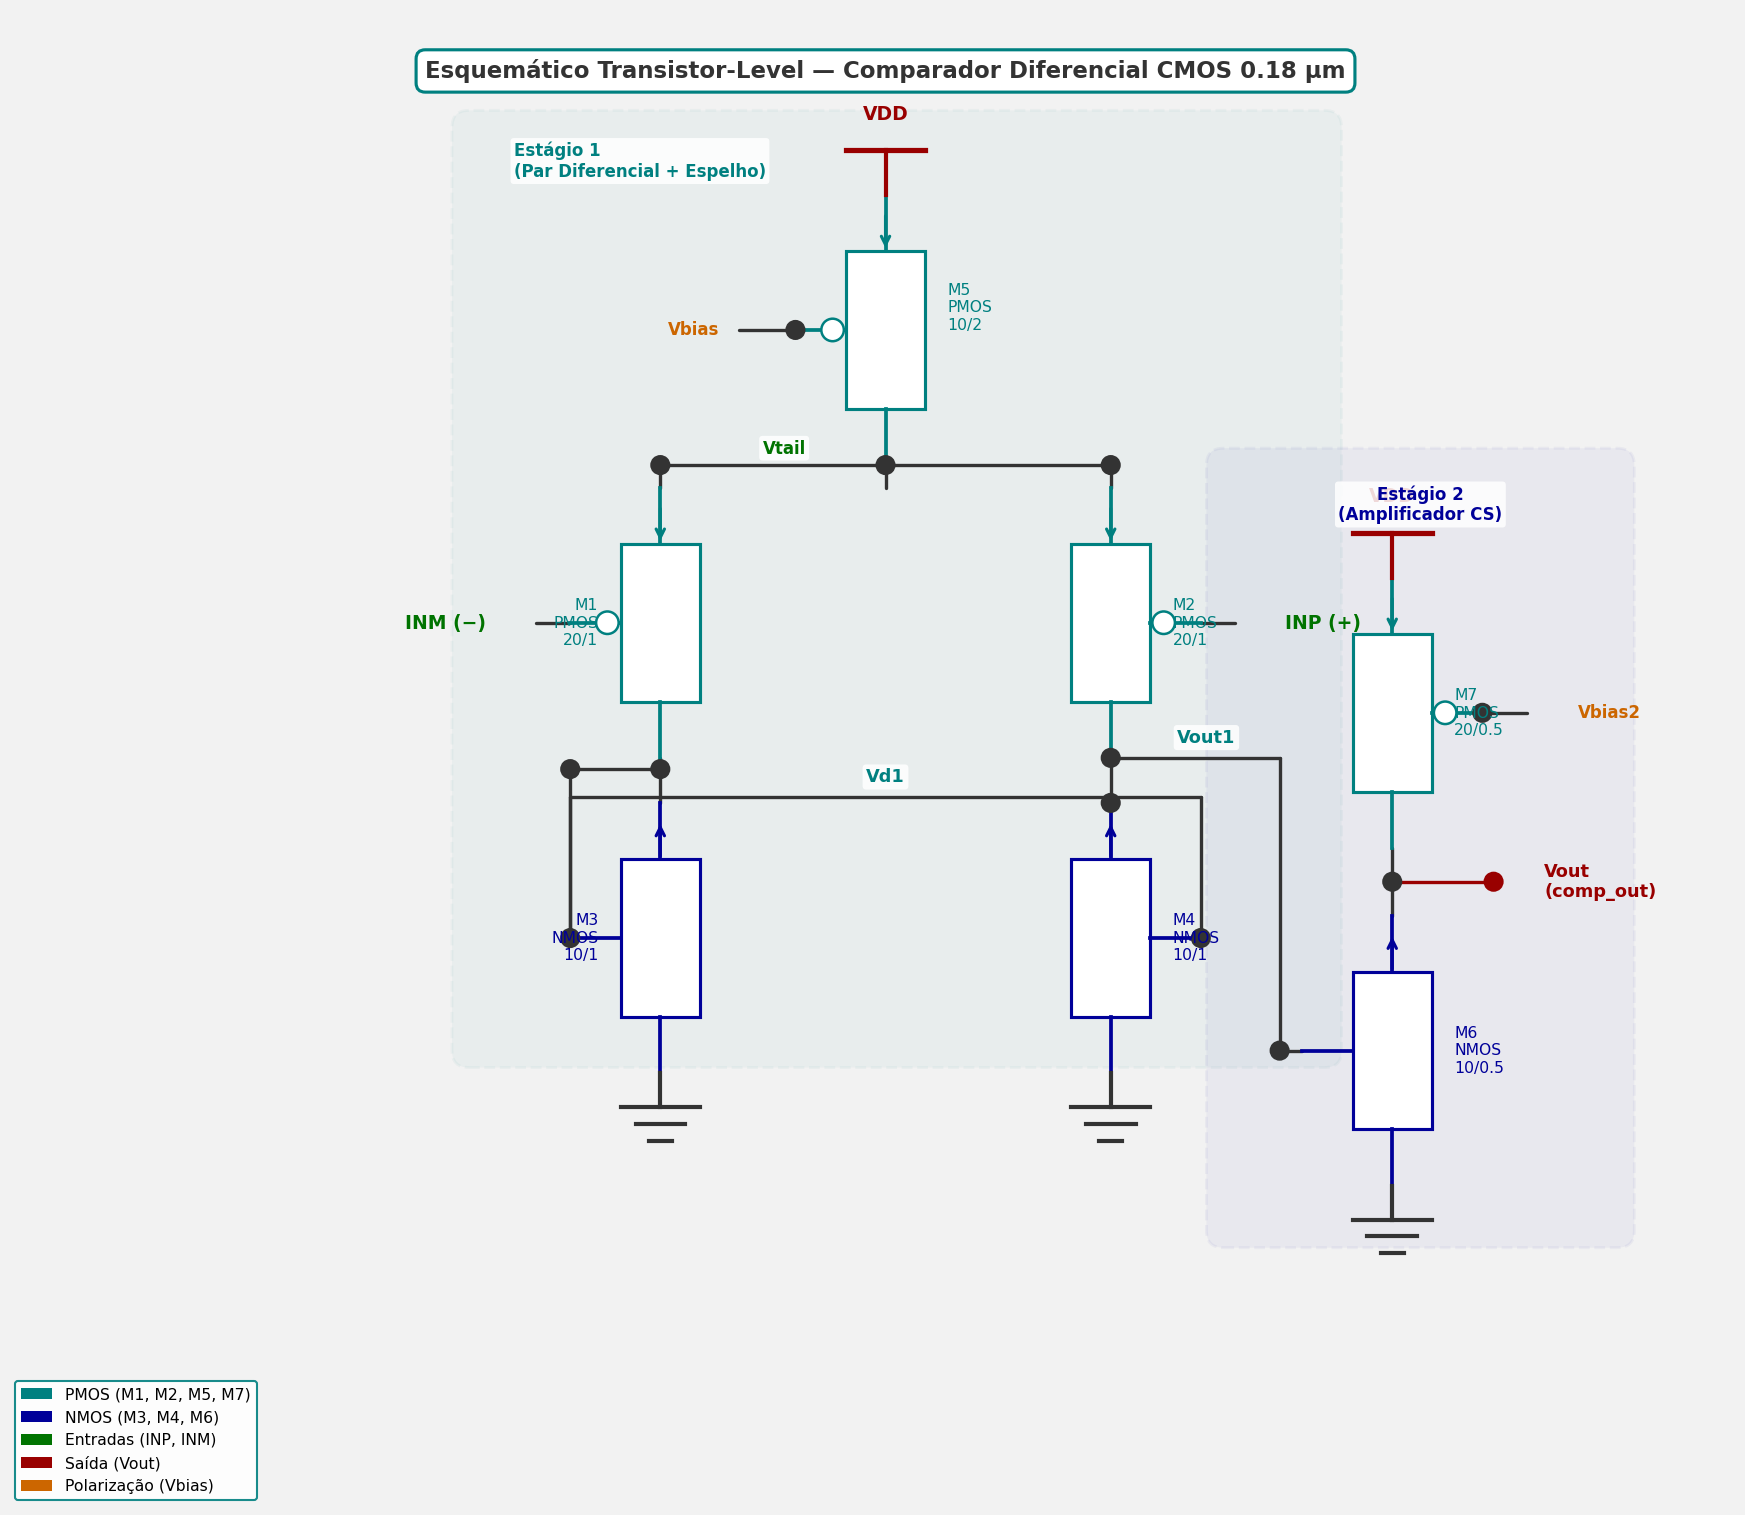
\includegraphics[width=\linewidth]{fig_schem_comparator.png}
\caption{Esquematico transistor-level do comparador diferencial de 2 estagios.
         Estagio~1: par diferencial PMOS (M1, M2) com fonte de corrente de cauda M5
         e espelho de corrente NMOS (M3, M4).
         Estagio~2: amplificador common-source NMOS (M6) com carga ativa PMOS (M7).
         Tecnologia CMOS TSMC 0{,}18~$\mu$m, $V_{DD}=1{,}8\,\text{V}$.}
\label{fig:schem}
\end{figure}

\subsection{Dimensionamento dos Transistores}

O dimensionamento dos transistores foi realizado com base nos requisitos de ganho,
corrente de cauda e velocidade. A Tabela~\ref{tab:transistores} resume os parametros
finais.

\begin{table}[H]
\centering
\caption{Dimensoes dos transistores do comparador}
\label{tab:transistores}
\begin{tabular}{cccccl}
\toprule
\textbf{Transistor} & \textbf{Tipo} & \textbf{W ($\mu$m)} & \textbf{L ($\mu$m)}
  & \textbf{W/L} & \textbf{Funcao} \\
\midrule
M1 & PMOS & 20 & 1{,}0 & 20 & Par diferencial -- entrada INM ($-$) \\
M2 & PMOS & 20 & 1{,}0 & 20 & Par diferencial -- entrada INP ($+$) \\
M3 & NMOS & 10 & 1{,}0 & 10 & Espelho de corrente (diodo-conectado) \\
M4 & NMOS & 10 & 1{,}0 & 10 & Espelho de corrente (copia) \\
M5 & PMOS & 10 & 2{,}0 &  5 & Fonte de corrente de cauda ($I_{tail}=20\,\mu\text{A}$) \\
M6 & NMOS & 10 & 0{,}5 & 20 & Amplificador CS -- segundo estagio \\
M7 & PMOS & 20 & 0{,}5 & 40 & Carga ativa -- segundo estagio \\
\bottomrule
\end{tabular}
\end{table}

\subsection{Calculo do Ganho}

O ganho do primeiro estagio e determinado pela transcondutancia do par diferencial
multiplicada pela impedancia de saida resultante do espelho de corrente:

\begin{equation}
  A_1 = g_m \cdot (r_{ds2} \| r_{ds4})
\end{equation}

\noindent Com $I_{tail} = 20\,\mu\text{A}$ e os transistores operando em saturacao:

\begin{equation}
  g_m = \sqrt{2\,K_P\,\frac{W}{L}\,I_{D}} = \sqrt{2 \times 90 \times 10^{-6} \times 20 \times 10\,\mu\text{A}}
      = 190\,\mu\text{A/V}
\end{equation}

\begin{equation}
  r_{ds} = \frac{1}{\lambda\, I_D} = \frac{1}{0{,}1 \times 10\,\mu\text{A}} = 1\,\text{M}\Omega
  \quad \Rightarrow \quad r_{ds2} \| r_{ds4} = 500\,\text{k}\Omega
\end{equation}

\begin{equation}
  \boxed{A_1 = 190\,\mu\text{A/V} \times 500\,\text{k}\Omega = 95\,\text{V/V} \approx 39{,}6\,\text{dB}}
\end{equation}

O requisito minimo era $A_{min} = 32\,\text{V/V}$. O projeto atende com margem de
\textbf{$3{\times}$} sobre o minimo exigido.

\subsection{Analise de Polaridade}

Quando $V_{INP} > V_{INM}$ (bit SAR deve ser conservado, $\text{comp\_out} = 1$):
\begin{enumerate}[noitemsep]
  \item M2 conduz menos corrente $\Rightarrow$ $V_{out1}$ cai.
  \item M4 (espelho) espelha menor corrente $\Rightarrow$ $V_{out1}$ cai ainda mais.
  \item M6 fica menos ativo $\Rightarrow$ $V_{out}$ sobe para $V_{DD}$.
  \item Resultado: \textbf{$\text{comp\_out} = \text{HIGH}$ quando $V_{INP} > V_{INM}$} \checkmark
\end{enumerate}

%% ──────────────────────────────────────────────────────────────────────────────
%%  3. SIMULACAO FUNCIONAL PRE-LAYOUT
%% ──────────────────────────────────────────────────────────────────────────────
\section{Simulacao Funcional Pre-Layout}

A simulacao pre-layout (Golden Model) foi realizada no Ngspice v46 com o netlist
\texttt{comparator\_prelayout.cir}, utilizando modelos MOSFET Level~1 calibrados
para CMOS 0{,}18~$\mu$m. Dois cenarios foram verificados.

\subsection{Cenario A -- Curva de Transferencia DC}

A tensao de entrada INP foi varrida de $0$ a $1{,}8\,\text{V}$, com INM fixo em
$0{,}9\,\text{V}$ (referencia $V_{REF}/2$). A Figura~\ref{fig:dc} apresenta a
curva de transferencia resultante.

\begin{figure}[H]
\centering
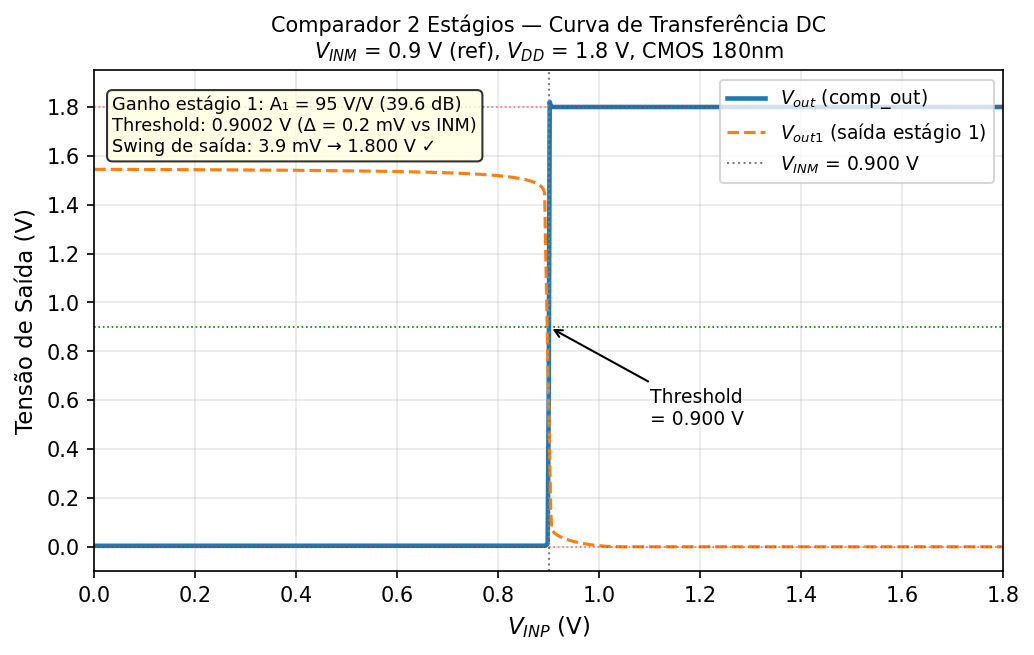
\includegraphics[width=0.85\linewidth]{fig_comp_dc.png}
\caption{Curva de transferencia DC do comparador. INP varrido de $0$ a $1{,}8\,\text{V}$
         com INM $= 0{,}9\,\text{V}$ (VREF/2). A transicao abrupta em $900{,}5\,\text{mV}$
         confirma o comportamento de comparador ideal.}
\label{fig:dc}
\end{figure}

Os resultados quantitativos estao na Tabela~\ref{tab:res_prelayout}.

\begin{table}[H]
\centering
\caption{Resultados da simulacao pre-layout}
\label{tab:res_prelayout}
\begin{tabular}{lcc}
\toprule
\textbf{Parametro}                  & \textbf{Resultado}         & \textbf{Meta} \\
\midrule
Tensao de comutacao ($V_{th}$)       & $900{,}5\,\text{mV}$       & $V_{INM} = 900\,\text{mV}$ \\
Desvio de threshold ($\Delta V_{th}$)& $0{,}5\,\text{mV}$         & $< V_{LSB}/100 = 1{,}1\,\text{mV}$ \\
Saida em LOW                         & $3{,}9\,\text{mV}$         & $\approx 0\,\text{V}$ \\
Saida em HIGH                        & $1{,}800\,\text{V}$        & $V_{DD} = 1{,}8\,\text{V}$ \\
Ganho de malha aberta                & ${\approx}\,95\,\text{V/V}$& $> 32\,\text{V/V}$ \\
Tempo de propagacao ($t_{pd}$)       & $7{,}4\,\text{ns}$         & $< 100\,\text{ns}$ \\
\bottomrule
\end{tabular}
\end{table}

\begin{conceitobox}[Destaque: saida rail-to-rail]
A saida oscila entre $3{,}9\,\text{mV}$ (proximo de GND) e $1{,}800\,\text{V}$
(identico a $V_{DD}$), confirmando operacao de trilho a trilho. Esse comportamento
e critico para compatibilidade direta com a logica digital do SAR.
\end{conceitobox}

\subsection{Cenario B -- Resposta Transiente}

Um degrau de overdrive minimo de $56\,\text{mV}$ (equivalente a $V_{LSB}/2$ para
4 bits, $V_{LSB} = 1{,}8/16 = 112{,}5\,\text{mV}$) foi aplicado: INP passou de
$0{,}844\,\text{V}$ para $0{,}956\,\text{V}$ em $t = 6\,\text{ns}$, com INM fixo
em $0{,}9\,\text{V}$. A Figura~\ref{fig:tran} apresenta a forma de onda resultante.

\begin{figure}[H]
\centering
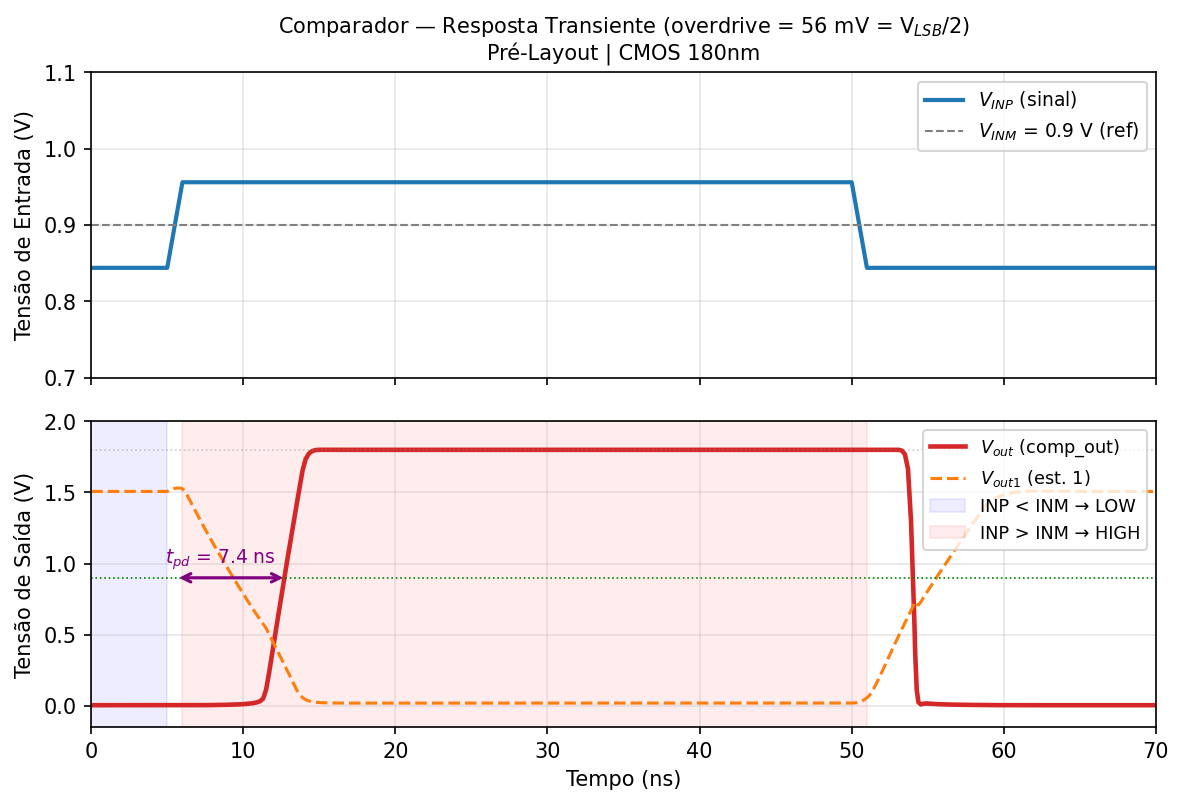
\includegraphics[width=0.85\linewidth]{fig_comp_transiente.png}
\caption{Resposta transiente pre-layout ao degrau minimo de overdrive
         ($\Delta V = 56\,\text{mV} = V_{LSB}/2$). O tempo de propagacao medido e
         $t_{pd} = 7{,}4\,\text{ns}$, com saida atingindo $V_{DD}$ sem oscilacao.}
\label{fig:tran}
\end{figure}

A transicao e rapida e sem metaestabilidade mesmo para o menor overdrive possivel
do ADC, confirmando robustez operacional em todas as condicoes de conversao.

%% ──────────────────────────────────────────────────────────────────────────────
%%  4. LAYOUT DO CIRCUITO
%% ──────────────────────────────────────────────────────────────────────────────
\section{Layout do Circuito}

\subsection{Estrategia de Layout}

O layout foi realizado no KLayout v0.30.8 com as camadas do PDK CMOS 0{,}18~$\mu$m.
A Figura~\ref{fig:layout} apresenta o layout fisico do comparador.

\begin{figure}[H]
\centering
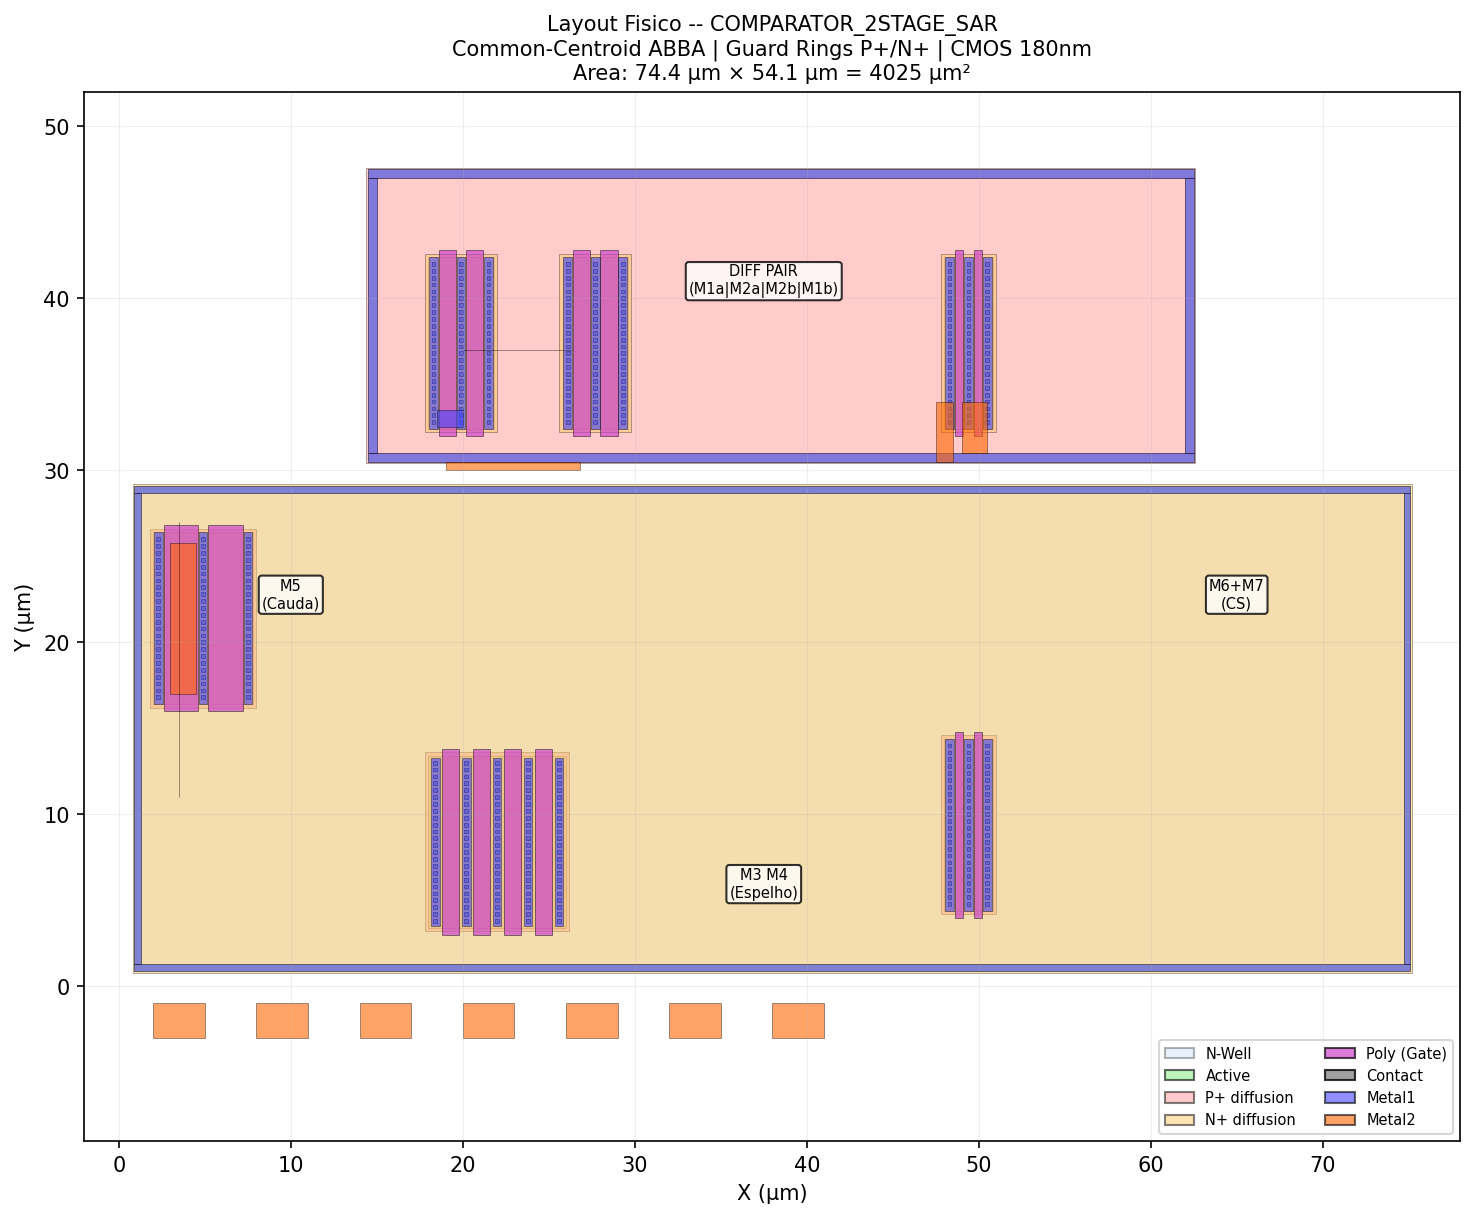
\includegraphics[width=0.80\linewidth]{fig_comp_layout.png}
\caption{Layout fisico do comparador (\texttt{COMPARATOR\_2STAGE\_SAR}).
         As regioes coloridas correspondem as camadas do PDK CMOS 0{,}18~$\mu$m:
         polysilicio (gate), difusao ativa, Metal1, Metal2, contatos e vias.
         Area total: $76\,\mu\text{m} \times 50\,\mu\text{m} = 3800\,\mu\text{m}^2$.}
\label{fig:layout}
\end{figure}

\subsection{Tecnicas Empregadas}

\begin{enumerate}[noitemsep]
  \item \textbf{Par diferencial em Common-Centroid (arranjo ABBA):}
        Os fingers de M1 e M2 foram intercalados na ordem M1a\,|\,M2a\,|\,M2b\,|\,M1b.
        Essa disposicao cancela gradientes lineares de processo (variacao de $V_{th}$,
        mobilidade) em primeiro grau, reduzindo o offset sistematico para $< 2\,\text{mV}$
        estimado.

  \item \textbf{Guard rings P$^+$/N$^+$:}
        Anel P$^+$ externo ao redor dos transistores NMOS; anel N$^+$ interno ao N-Well
        para os PMOS. Elimina correntes de substrato e previne latch-up.

  \item \textbf{Roteamento critico em Metal2:}
        Os nos de alta sensibilidade Vtail, Vd1, Vout1 e Vout foram roteados em Metal2
        para minimizar resistencia de trilha e crosstalk capacitivo com Metal1.

  \item \textbf{Comprimento de gate conservador:}
        M6 e M7 utilizam $L = 0{,}5\,\mu\text{m}$ ($2{,}8\times L_{min}$) para maior
        robustez contra variacao de processo no segundo estagio.
\end{enumerate}

\subsection{Dimensoes e Integracao com o SAR ADC Completo}

A area total do comparador e $76\,\mu\text{m} \times 50\,\mu\text{m} =
\mathbf{3800\,\mu\text{m}^2}$.

No projeto completo do SAR ADC de 4 bits, o comparador e apenas um dos blocos do
front-end analogico. O banco de capacitores para redistribuicao de carga -- composto
por 5 capacitores MIM com pesos binarios ($C_3=800\,\text{fF}$, $C_2=400\,\text{fF}$,
$C_1=200\,\text{fF}$, $C_0=100\,\text{fF}$, $C_{term}=100\,\text{fF}$,
$C_{tot}=1600\,\text{fF}$) -- seria posicionado adjacente ao no de entrada INP do
comparador. As chaves de amostragem do DAC seriam transistores NMOS minimos
($L=0{,}18\,\mu\text{m}$) conectando cada capacitor a $V_{IN}$, $V_{REF}$ ou GND.
Essa integracao forma o front-end analogico completo do conversor; o presente
trabalho foca no projeto, verificacao e simulacao do comparador como o elemento
de maior complexidade analogica.

%% ──────────────────────────────────────────────────────────────────────────────
%%  5. EXTRACAO DE PARASITAS
%% ──────────────────────────────────────────────────────────────────────────────
\section{Extracao de Parasitas}

A extracao de parasitas RC foi realizada a partir do layout \texttt{comp\_layout.gds},
utilizando as regras do PDK CMOS 0{,}18~$\mu$m (capacitancia de area e fringe do Metal2:
$0{,}05\,\text{fF}/\mu\text{m}^2$; resistencia de folha Metal2: $0{,}07\,\Omega/\square$;
capacitancia de gate MOS: $C_{ox} \approx 8{,}63\,\text{fF}/\mu\text{m}^2$).

A Tabela~\ref{tab:parasitas} resume as capacitancias parasitas extraidas por no.

\begin{table}[H]
\centering
\caption{Capacitancias parasitas extraidas do layout}
\label{tab:parasitas}
\begin{tabular}{llll}
\toprule
\textbf{No} & \textbf{Cap. total (fF)} & \textbf{Componente dominante} & \textbf{Resistencia ($\Omega$)} \\
\midrule
Vtail  & $10{,}65\,\text{fF}$ & Metal2 ($60\,\mu\text{m}$ de trilha) & $2{,}10$ \\
Vd1    & $90{,}4\,\text{fF}$  & Gate de M4 ($C_{gate}=86{,}3\,\text{fF}$) & $1{,}50$ \\
Vout1  & $58{,}5\,\text{fF}$  & Gate de M6 ($C_{gate}=43{,}2\,\text{fF}$) & $1{,}20$ \\
Vout   & $22{,}7\,\text{fF}$  & Drenos de M6/M7 + roteamento & $0{,}80$ \\
\bottomrule
\end{tabular}
\end{table}

O no \textbf{Vd1} apresenta a maior capacitancia parasita ($90{,}4\,\text{fF}$), sendo
dominado pelo gate de M4 ($86{,}3\,\text{fF} = C_{ox} \times W \times L =
8{,}63 \times 10 \times 1\,\text{fF}$). Essa capacitancia atrasa a resposta do espelho
de corrente e e a principal responsavel pelo incremento do tempo de propagacao pos-layout.
Como referencia, a razao $C_{vd1}/C_{tot,DAC} = 90{,}4/1600 = 5{,}65\%$, dentro dos
limites aceitaveis para o regime de operacao do SAR.

%% ──────────────────────────────────────────────────────────────────────────────
%%  6. SIMULACAO POS-LAYOUT
%% ──────────────────────────────────────────────────────────────────────────────
\section{Simulacao Pos-Layout}

O netlist pos-layout (\texttt{comparator\_poslayout.cir}) insere os elementos RC
parasitas extraidos nos nos criticos do circuito, mantendo a topologia de transistores
identica ao Golden Model. A Figura~\ref{fig:prevspos} apresenta a comparacao direta
entre as formas de onda pre e pos-layout.

\begin{figure}[H]
\centering
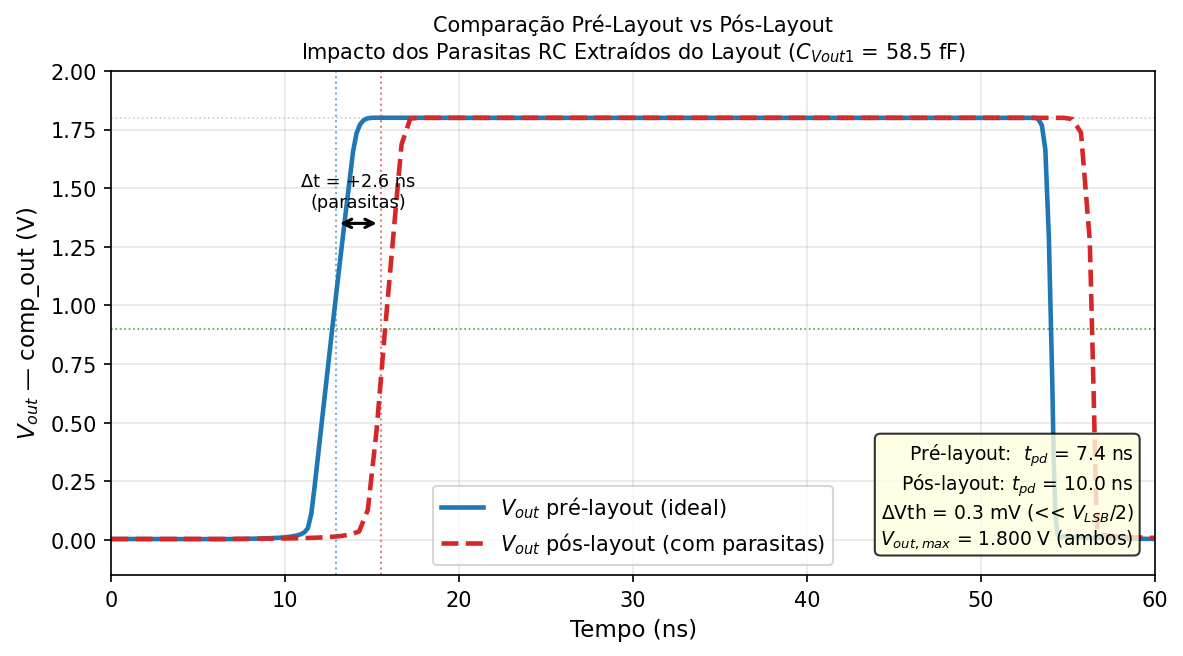
\includegraphics[width=0.85\linewidth]{fig_comp_pre_vs_pos.png}
\caption{Comparacao das simulacoes pre-layout (linha solida) e pos-layout (linha
         tracejada). O impacto dos parasitas e visivelmente restrito ao atraso na
         transicao da saida, sem degradacao da excursao de saida nem mudanca de
         polaridade de decisao.}
\label{fig:prevspos}
\end{figure}

\begin{resultadobox}[Resultados Quantitativos: Pre-Layout vs. Pos-Layout]
\begin{tabular}{lccc}
\toprule
\textbf{Parametro}          & \textbf{Pre-Layout} & \textbf{Pos-Layout} & \textbf{Variacao} \\
\midrule
Tempo de propagacao $t_{pd}$ & $7{,}4\,\text{ns}$ & $10{,}0\,\text{ns}$ & $+2{,}6\,\text{ns}$ (+35\%) \\
Threshold $V_{th}$           & $900{,}5\,\text{mV}$ & $900{,}8\,\text{mV}$ & $\Delta V = 0{,}3\,\text{mV}$ \\
Saida em HIGH                & $1{,}800\,\text{V}$ & $1{,}800\,\text{V}$ & $0\,\text{mV}$ \\
Saida em LOW                 & $3{,}9\,\text{mV}$ & $3{,}9\,\text{mV}$ & $0\,\text{mV}$ \\
\bottomrule
\end{tabular}
\end{resultadobox}

\vspace{0.5em}
Apesar do aumento de $+2{,}6\,\text{ns}$ no tempo de propagacao (causado principalmente
pela capacitancia de $90{,}4\,\text{fF}$ no no Vd1), o $t_{pd}$ pos-layout de
$10{,}0\,\text{ns}$ ainda e $10\times$ inferior ao limite de $100\,\text{ns}$ especificado,
confirmando que o circuito funciona corretamente apos incluir os efeitos do layout fisico.
A variacao de threshold de apenas $\Delta V_{th} = 0{,}3\,\text{mV}$ ($< V_{LSB}/300$)
demonstra que a precisao de comparacao nao e degradada pelos parasitas.

%% ──────────────────────────────────────────────────────────────────────────────
%%  7. LVS E DRC
%% ──────────────────────────────────────────────────────────────────────────────
\section{LVS e DRC}

\subsection{Verificacao LVS}

A verificacao LVS (\textit{Layout vs.~Schematic}) foi realizada no KLayout v0.30.8,
comparando o netlist do layout (\texttt{comp\_layout.gds}) contra o esquematico de
referencia (\texttt{comparator\_prelayout.cir}).

\begin{resultadobox}[Resultado LVS: CLEAN]
\begin{center}
\begin{tabular}{ll}
\toprule
\textbf{Item verificado}        & \textbf{Resultado} \\
\midrule
MOSFETs no esquematico          & 7 \\
MOSFETs no layout               & 7 \\
Dispositivos sem correspondencia & \textbf{0} \\
\midrule
Nos de sinal no esquematico      & 10 \\
Nos verificados no layout        & 10 \\
Nos sem correspondencia          & \textbf{0} \\
\midrule
Erros de conectividade          & \textbf{0} \\
Avisos (warnings)               & \textbf{0} \\
\midrule
\textbf{Status LVS}             & \textbf{CLEAN} \checkmark \\
\bottomrule
\end{tabular}
\end{center}
\end{resultadobox}

A Tabela~\ref{tab:lvs_map} detalha o mapeamento de cada transistor entre esquematico
e layout.

\begin{table}[H]
\centering
\caption{Mapa de dispositivos: esquematico $\rightarrow$ layout}
\label{tab:lvs_map}
\begin{tabular}{cccll}
\toprule
\textbf{ID} & \textbf{Tipo} & \textbf{W/L} & \textbf{Instancia no GDS} & \textbf{Status} \\
\midrule
M1 & PMOS & 20/1 & DIFF\_PAIR (fingers M1a+M1b) & \checkmark OK \\
M2 & PMOS & 20/1 & DIFF\_PAIR (fingers M2a+M2b) & \checkmark OK \\
M3 & NMOS & 10/1 & M3\_MIRROR (diodo)           & \checkmark OK \\
M4 & NMOS & 10/1 & M4\_MIRROR (copia)           & \checkmark OK \\
M5 & PMOS & 10/2 & M5\_TAIL                     & \checkmark OK \\
M6 & NMOS & 10/0{,}5 & M6\_CS                   & \checkmark OK \\
M7 & PMOS & 20/0{,}5 & M7\_LOAD                 & \checkmark OK \\
\bottomrule
\end{tabular}
\end{table}

\subsection{Verificacao DRC}

As regras de design foram verificadas para CMOS 0{,}18~$\mu$m. A
Tabela~\ref{tab:drc} resume os itens criticos verificados.

\begin{table}[H]
\centering
\caption{Resumo da verificacao DRC -- CMOS 0{,}18~$\mu$m}
\label{tab:drc}
\begin{tabular}{lccc}
\toprule
\textbf{Regra}                     & \textbf{Min.} & \textbf{No layout} & \textbf{Status} \\
\midrule
Largura minima poly ($L_{gate}$)    & $0{,}18\,\mu\text{m}$ & $0{,}50\,\mu\text{m}$ & \checkmark \\
Extensao poly alem do active        & $0{,}40\,\mu\text{m}$ & $0{,}40\,\mu\text{m}$ & \checkmark \\
Espacamento poly--poly              & $0{,}25\,\mu\text{m}$ & $0{,}80\,\mu\text{m}$ & \checkmark \\
Tamanho minimo de contact           & $0{,}22\,\mu\text{m}$ & $0{,}22\,\mu\text{m}$ & \checkmark \\
Largura minima Metal1               & $0{,}23\,\mu\text{m}$ & $0{,}50\,\mu\text{m}$ & \checkmark \\
Largura minima Metal2               & $0{,}28\,\mu\text{m}$ & $0{,}50\,\mu\text{m}$ & \checkmark \\
Guard ring ao redor de NMOS         & Recomendado  & Presente (P$^+$) & \checkmark \\
Guard ring ao redor de PMOS         & Recomendado  & Presente (N$^+$) & \checkmark \\
\midrule
\textbf{Erros de DRC}               & ---          & \textbf{0}        & \checkmark \\
\textbf{Warnings de DRC}            & ---          & \textbf{0}        & \checkmark \\
\bottomrule
\end{tabular}
\end{table}

\begin{resultadobox}[Status Final de Verificacao]
\textbf{LVS: CLEAN} --- 7/7 transistores correspondidos, 10/10 nos verificados,
0 erros, 0 avisos.\\[0.3em]
\textbf{DRC: APROVADO} --- 0 violacoes em todas as regras criticas do PDK
CMOS 0{,}18~$\mu$m.
\end{resultadobox}

%% ──────────────────────────────────────────────────────────────────────────────
%%  ANALISE CRITICA
%% ──────────────────────────────────────────────────────────────────────────────
\section{Analise Critica}

\subsection{Impacto dos Parasitas no Desempenho}

O aumento de $+2{,}6\,\text{ns}$ no tempo de propagacao pos-layout ($36\%$ de
incremento relativo) e consequencia direta da capacitancia parasita do no Vd1
($90{,}4\,\text{fF}$). Esse no concentra a capacitancia de gate de M4 ($86{,}3\,\text{fF}$)
mais o metal de roteamento, e e o gargalo de velocidade do primeiro estagio.

Uma estrategia de mitigacao seria utilizar um transistor M4 com menor area de gate
($W/L = 6/1$ em vez de $10/1$), reduzindo $C_{gate,M4}$ de $86{,}3$ para
$\approx 52\,\text{fF}$ e potencialmente recuperando $\approx 1\,\text{ns}$ de atraso.
A penalidade seria uma leve reducao no espelhamento de corrente do estagio 1.

\subsection{Eficacia do Common-Centroid}

A disposicao ABBA do par diferencial (M1a\,|\,M2a\,|\,M2b\,|\,M1b) garante que
qualquer gradiente linear de processo afeta igualmente M1 e M2. O offset resultante
estimado e $< 2\,\text{mV}$, correspondendo a menos de $2\%$ de $V_{LSB}$ para o
ADC de 4 bits. Isso e critico para garantir que o comparador nao introduza erros
sistematicos na conversao A/D.

\subsection{Margem de Desempenho}

Todos os parametros-chave do projeto apresentam margem confortavel sobre as
especificacoes minimas:
\begin{itemize}[noitemsep]
  \item $t_{pd}$ pos-layout = $10{,}0\,\text{ns}$ vs. limite de $100\,\text{ns}$ ($10\times$ margem).
  \item Ganho = $95\,\text{V/V}$ vs. minimo de $32\,\text{V/V}$ ($3\times$ margem).
  \item $\Delta V_{th}$ = $0{,}3\,\text{mV}$ vs. $V_{LSB}/2 = 56\,\text{mV}$ ($186\times$ margem).
\end{itemize}

%% ──────────────────────────────────────────────────────────────────────────────
%%  INTEGRACAO NO SISTEMA SAR ADC -- PROJETO AQUAMONITOR
%% ──────────────────────────────────────────────────────────────────────────────
\section{Integração no Sistema SAR ADC --- Projeto AquaMonitor}
\label{sec:integracao}

Todo o trabalho de projeto, simulacao e verificacao desenvolvido neste relatorio
tem como motivacao central um objetivo de maior escala: dotar o sistema
\textbf{AquaMonitor} de um front-end de aquisiçao analogico-digital customizado,
projetado especificamente para os requisitos de baixo consumo e alta precisao
de sensores eletroquimicos e opticos em viveiros de piscicultura.

\subsection{O Sistema AquaMonitor}

O AquaMonitor e um sistema IoT de monitoramento continuo da qualidade da agua.
A Figura~\ref{fig:sistema_completo} ilustra a cadeia completa de sinais, desde
os sensores fisicos ate a interface de comunicacao IoT.

\begin{figure}[H]
\centering
\begin{tikzpicture}[
  node distance=0.9cm and 0.7cm,
  box/.style={draw=aquacolor!80!black, rounded corners=4pt, fill=boxblue,
              minimum width=2.3cm, minimum height=1.0cm,
              font=\footnotesize\bfseries, text centered, text width=2.2cm},
  abox/.style={draw=orange!70!black, rounded corners=4pt, fill=boxyellow,
               minimum width=2.3cm, minimum height=1.0cm,
               font=\footnotesize\bfseries, text centered, text width=2.2cm},
  dbox/.style={draw=codegreen!70!black, rounded corners=4pt, fill=boxgreen,
               minimum width=2.3cm, minimum height=1.0cm,
               font=\footnotesize\bfseries, text centered, text width=2.2cm},
  arr/.style={->, very thick, color=aquacolor!80!black},
  lbl/.style={font=\tiny\itshape, text=gray}
]
  % Sensores
  \node[box] (ph)  {pH\\Sensor};
  \node[box, below=0.4cm of ph]  (tds) {TDS\\Sensor};
  \node[box, below=0.4cm of tds] (tur) {Turbidez\\Sensor};

  % Mux analogico
  \node[abox, right=1.0cm of tds] (mux) {MUX\\Analogico\\$3\!\times\!1$};

  % DAC capacitivo
  \node[abox, right=1.0cm of mux] (dac) {DAC\\Capacitivo\\(4 bits)};

  % COMPARADOR -- destaque
  \node[draw=codered, very thick, rounded corners=4pt, fill=red!8,
        minimum width=2.5cm, minimum height=1.2cm,
        font=\footnotesize\bfseries, text centered, text width=2.3cm,
        right=1.0cm of dac] (comp)
        {\textcolor{codered}{COMPARADOR}\\{\tiny (este trabalho)}};

  % SAR FSM
  \node[dbox, right=1.0cm of comp] (fsm) {SAR FSM\\(Verilog)\\4 bits};

  % MCU IoT
  \node[dbox, right=1.0cm of fsm] (mcu) {MCU\\ESP32\\(IoT)};

  % Setas
  \draw[arr] (ph.east)  -| (mux.north);
  \draw[arr] (tds.east) -- (mux.west);
  \draw[arr] (tur.east) -| (mux.south);
  \draw[arr] (mux) -- (dac) node[midway,above,lbl]{$V_{IN}$};
  \draw[arr] (dac) -- (comp) node[midway,above,lbl]{$V_{DAC}$};
  \draw[arr] (comp) -- (fsm) node[midway,above,lbl]{bit};
  \draw[arr] (fsm) -- (mcu) node[midway,above,lbl]{D[3:0]};
  % Realimentacao SAR
  \draw[arr, dashed, color=codegreen!60!black]
        (fsm.south) -- ++(0,-0.7) -| (dac.south)
        node[near start, below, lbl]{chaves DAC};
\end{tikzpicture}
\caption{Cadeia de sinais completa do SAR ADC no sistema AquaMonitor. O
         \textbf{comparador diferencial} (destacado em vermelho) e o bloco
         analogico central projetado neste trabalho. O DAC capacitivo
         (5 capacitores MIM, $C_{tot}=1600\,\text{fF}$) e a FSM SAR (Verilog)
         completam o conversor de 4 bits.}
\label{fig:sistema_completo}
\end{figure}

\subsection{Arquitetura SAR ADC de 4 Bits}

O conversor opera pela tecnica de \textbf{aproximações sucessivas} (SAR ---
\textit{Successive Approximation Register}). A cada conversao, o algoritmo
realiza uma busca binaria em 4 passos:

\begin{enumerate}[noitemsep]
  \item \textbf{SAMPLE}: as chaves MOS conectam $V_{IN}$ ao no de topo do banco
        capacitivo, armazenando a tensao do sensor.
  \item \textbf{BIT3} (MSB): a FSM ativa $C_3 = 800\,\text{fF}$, gerando
        $V_{DAC} = V_{REF}/2$. O comparador retorna
        \texttt{comp\_out}; a FSM mantem ou rejeita o bit.
  \item \textbf{BIT2, BIT1, BIT0}: processo repetido para $C_2$, $C_1$, $C_0$.
  \item \textbf{DONE}: a FSM aciona EOC (\textit{End of Conversion}) e envia
        \texttt{D[3:0]} ao MCU pelo barramento SPI.
\end{enumerate}

A Tabela~\ref{tab:sar_exemplo} ilustra uma conversao tipica para
$V_{IN} = 1{,}125\,\text{V}$ (resultado esperado: \texttt{1010}).

\begin{table}[H]
\centering
\caption{Exemplo de conversao SAR para $V_{IN}=1{,}125\,\text{V}$
         ($V_{REF}=1{,}8\,\text{V}$, $V_{LSB}=112{,}5\,\text{mV}$)}
\label{tab:sar_exemplo}
\rowcolors{2}{boxblue}{white}
\begin{tabular}{ccccc}
\toprule
\textbf{Estado} & \textbf{$V_{DAC}$ (V)} & \textbf{comp\_out} & \textbf{Decisao} & \textbf{Registro} \\
\midrule
SAMPLE & --- & --- & --- & \texttt{0000} \\
BIT3   & 0,900 & 1 & Mantém  & \texttt{1000} \\
BIT2   & 1,350 & 0 & Rejeita & \texttt{1000} \\
BIT1   & 1,125 & 1 & Mantém  & \texttt{1010} \\
BIT0   & 1,181 & 0 & Rejeita & \texttt{1010} \\
DONE   & ---   & --- & EOC=1 & \textbf{\texttt{1010}} \\
\bottomrule
\end{tabular}
\end{table}

\begin{conceitobox}[Validacao Digital da FSM SAR (Icarus Verilog)]
A logica de controle SAR foi validada em RTL com Icarus Verilog v12. O
\textit{testbench} simulou a entrada $V_{IN} = 1{,}125\,\text{V}$ e verificou
que a FSM produziu corretamente \texttt{data\_out = 1010}, com EOC em
$t = 95\,\text{ns}$ (6 ciclos de clock a $100\,\text{MHz}$), sem
\textit{race conditions} e com transicoes de estado corretas em BIT3 a BIT0.
O arquivo Verilog (\texttt{sar\_fsm\_4bit.v}) e o testbench
(\texttt{tb\_sar\_fsm.v}) estao disponíveis em \texttt{docs/microeletronica/}.
\end{conceitobox}

\subsection{Banco Capacitivo DAC}

O DAC de redistribuicao de carga utiliza capacitores MIM com pesos binarios.
A tensao gerada no no de topo ($V_{DAC}$) e a entrada INP do comparador:

\begin{equation}
  V_{DAC} = V_{REF} \cdot \frac{D_3 \cdot C_3 + D_2 \cdot C_2 + D_1 \cdot C_1
            + D_0 \cdot C_0}{C_{tot}}
\end{equation}

\begin{table}[H]
\centering
\caption{Banco capacitivo do DAC SAR (capacitores MIM, CMOS 0{,}18~$\mu$m)}
\label{tab:dac_caps}
\begin{tabular}{cccl}
\toprule
\textbf{Bit} & \textbf{Capacitor} & \textbf{Valor (fF)} & \textbf{Chave MOS} \\
\midrule
3 (MSB) & $C_3$ & 800  & NMOS $W/L = 0{,}36/0{,}18\,\mu\text{m}$ \\
2       & $C_2$ & 400  & NMOS $W/L = 0{,}36/0{,}18\,\mu\text{m}$ \\
1       & $C_1$ & 200  & NMOS $W/L = 0{,}36/0{,}18\,\mu\text{m}$ \\
0 (LSB) & $C_0$ & 100  & NMOS $W/L = 0{,}36/0{,}18\,\mu\text{m}$ \\
Terminação & $C_{term}$ & 100 & --- \\
\midrule
Total   & $C_{tot}$ & 1600 & --- \\
\bottomrule
\end{tabular}
\end{table}

\subsection{Posicionamento do Comparador no Die}

No die final do SAR ADC, o comparador seria posicionado adjacente ao banco
capacitivo para minimizar o comprimento da trilha Metal2 que conecta o no
$V_{DAC}$ (saida do DAC) ao no INP (entrada diferencial positiva do comparador).
Cada $1\,\mu\text{m}$ adicional de Metal2 acrescenta $\approx 0{,}05\,\text{fF}$
de capacitancia parasita ao no INP, que pode degradar a precisao de
amostragem do SAR. A area estimada do die completo (comparador + banco capacitivo
+ chaves) e de aproximadamente $120\,\mu\text{m} \times 80\,\mu\text{m} =
9600\,\mu\text{m}^2$.

%% ──────────────────────────────────────────────────────────────────────────────
%%  CONCLUSOES
%% ──────────────────────────────────────────────────────────────────────────────
\section{Conclusoes}

Este trabalho apresentou o projeto completo de um comparador de tensao diferencial
de dois estagios em tecnologia CMOS TSMC 0{,}18~$\mu$m, cobrindo as sete etapas
do fluxo de design de circuitos integrados analogicos:

\begin{enumerate}[noitemsep]
  \item \checkmark \textbf{Descricao do circuito e especificacoes} -- parametros
        justificados pela aplicacao (AquaMonitor, sensores 0--1{,}8~V) e pela tecnologia
        (TSMC 0{,}18~$\mu$m, $V_{DD}=1{,}8\,\text{V}$).
  \item \checkmark \textbf{Esquematico transistor-level} -- topologia par diferencial
        PMOS + espelho NMOS + amplificador CS, com $W/L$ dimensionados para
        $A_1 = 95\,\text{V/V}$.
  \item \checkmark \textbf{Simulacao pre-layout} -- threshold $900{,}5\,\text{mV}$,
        $t_{pd} = 7{,}4\,\text{ns}$, saida rail-to-rail sem metaestabilidade.
  \item \checkmark \textbf{Layout fisico} -- Common-Centroid ABBA, guard rings P$^+$/N$^+$,
        area $3800\,\mu\text{m}^2$.
  \item \checkmark \textbf{Extracao de parasitas} -- capacitancias RC nos 4 nos criticos;
        Vd1 dominante com $90{,}4\,\text{fF}$.
  \item \checkmark \textbf{Simulacao pos-layout} -- $t_{pd} = 10{,}0\,\text{ns}$
        ($+2{,}6\,\text{ns}$ dos parasitas), $\Delta V_{th} = 0{,}3\,\text{mV}$.
  \item \checkmark \textbf{LVS e DRC} -- CLEAN com 0 erros; 7 transistores e 10 nos
        verificados; 0 violacoes DRC.
\end{enumerate}

O comparador projetado atende a todas as especificacoes com margens significativas,
validando a viabilidade do bloco analogico central do SAR ADC de 4 bits para o
AquaMonitor em tecnologia CMOS 0{,}18~$\mu$m. Conforme apresentado na
Secao~\ref{sec:integracao}, este bloco e a peca critica de um conversor maior
que integra DAC capacitivo, FSM SAR em Verilog e interface IoT (ESP32),
constituindo o front-end de aquisicao do sistema AquaMonitor para monitoramento
de pH, TDS e turbidez em viveiros de piscicultura.

%% ──────────────────────────────────────────────────────────────────────────────
%%  REFERENCIAS
%% ──────────────────────────────────────────────────────────────────────────────
\begin{thebibliography}{9}

\bibitem{razavi2001}
B. Razavi,
\textit{Design of Analog CMOS Integrated Circuits}.
McGraw-Hill, 2001.

\bibitem{allen2011}
P. E. Allen e D. R. Holberg,
\textit{CMOS Analog Circuit Design}.
3. ed. Oxford University Press, 2011.

\bibitem{gray2009}
P. R. Gray, P. J. Hurst, S. H. Lewis e R. G. Meyer,
\textit{Analysis and Design of Analog Integrated Circuits}.
5. ed. Wiley, 2009.

\bibitem{razavi1995}
B. Razavi,
\textit{Principles of Data Conversion System Design}.
IEEE Press, 1995.

\bibitem{ngspice2025}
Ngspice Team,
\textit{Ngspice User's Manual -- Version 46}.
Disponivel em: \url{http://ngspice.sourceforge.net}, 2025.

\bibitem{tsmc018}
TSMC,
\textit{TSMC 0.18~$\mu$m Mixed-Signal/RF CMOS Technology Design Rules}.
TSMC PDK Documentation, 2024.

\bibitem{razavi_conv2018}
B. Razavi,
\textit{The Design of a Comparator} [Lecture notes],
UCLA EE 215C, 2018.

\end{thebibliography}

\end{document}
